\section{Electrical reproduction of sound}

\bi
\i A basic understanding of electricity and magnetism is 
needed to describe the functioning of musical recording 
and reproduction equipment.

\i Here, we briefly describe electrical circuits (voltage, current,
resistance, power, $\cdots$) and also Faraday's law of induction, 
which underlies the operation of microphones and loudspeakers.

\ei

%%%%%%%%%%%%%%%%%%%%%%%%%%%%%%%%%%%%%%%%%%%%%%%%%%%%%%%%%%%
\subsection{Basic electricity}

\bi

\i When a voltage source (such as a battery) is connected to a 
load (such as a flashlight bulb) via a closed path (called a
circuit), an electric current flows (electric charges in motion).

\i The voltage is denoted by $V$ and is measured in volt (V).
The load has a {\em resistance}, denoted by $R$, which is 
measured in Ohm ($\Omega$).
The current is denoted by $I$ and is measured in Amp\`ere or 
Amp (A).

\i For certain materials, $V$, $I$, and $R$ are related by 
%
\be
R=V/I\quad{\rm or,\ equivalently,}\quad 
V= IR
\ee
%
This is called {\em Ohm's law of electricity}, not to be confused
with {\em Ohm's law of hearing}, even though it's by the same guy.

\i For a battery, which has a {\em polarity} ($+$ and 
$-$ terminals), the current $I$ flows in only one direction, 
which we take to be from the $+$ terminal of the battery 
to the $-$ terminal.
This is called a {\em direct current} (DC) circuit.
(See the left-hand panel of Figure~\ref{f:circuits_DC_AC}.)
%
\begin{figure}[htbp]
\begin{center}
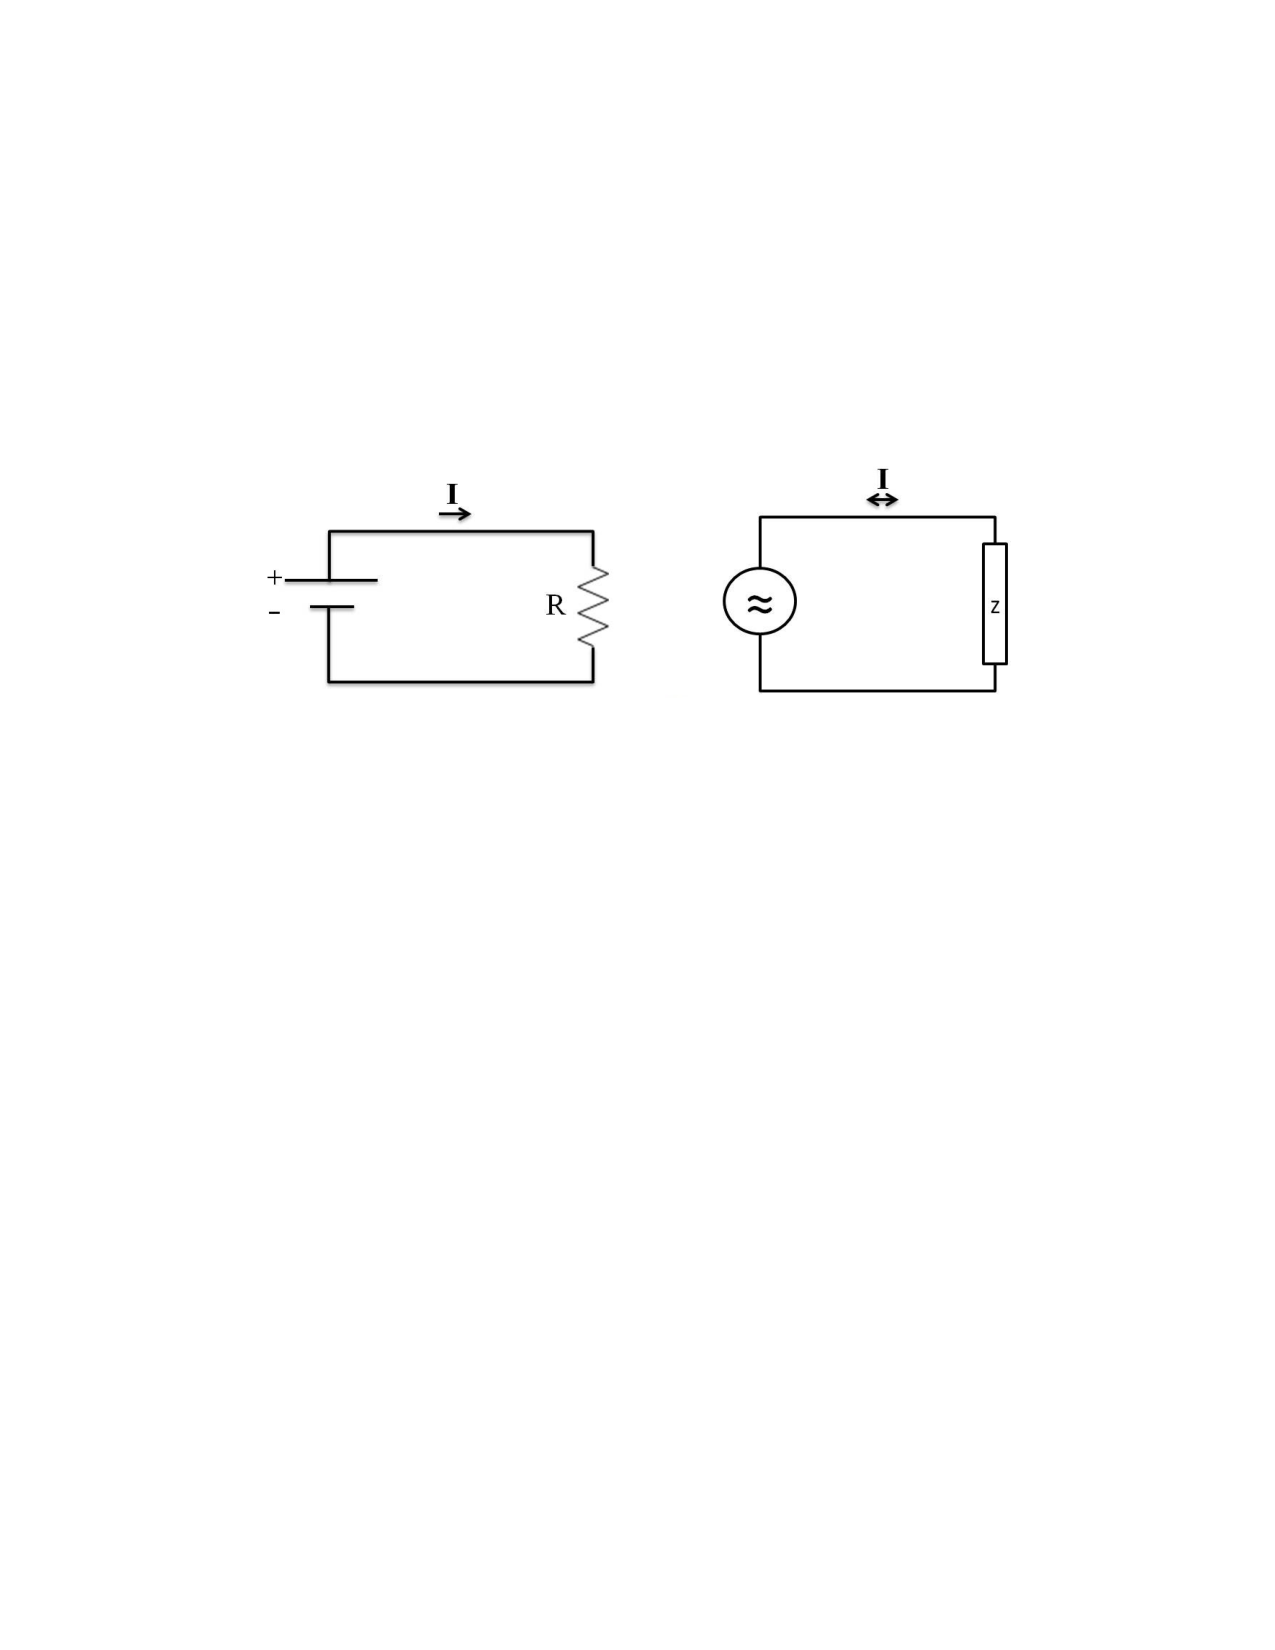
\includegraphics[width=0.75\textwidth]{circuits_DC_AC}
\caption{Left: Direct current (DC) circuit, consisting
of a voltage source $V$ and load having resistance $R$.
Right: Alternating current (AC) circuit, consisting of
a voltage source $V$ and load having impedance $Z$.
For a DC circuit, the current $I$ flows in only one direction.
For an AC circuit, the current $I$ flows alternately clockwise and
counterclockwise around the circuit.
(Figures from ``PHYS 1406: Physics of Sound \& Music" 
Course Guide by Prof.~Borst.)}
\label{f:circuits_DC_AC}
\end{center}
\end{figure}

\i For a household wall outlet, the voltage $V$ alternates
sinusoidally with time (60~cycle/sec or 60~Hz), 
producing a current $I$ that 
also alternates sinusoidally, traveling both clockwise and 
counterclockwise around the circuit.
Such a circuit is called an {\em alternating current} (AC) circuit.
(See the right-hand panel of Figure~\ref{f:circuits_DC_AC}.)

\i For AC circuits, there is a relation 
%
\be
V = I Z
\ee
%
which is similar to Ohm's law, but it involves the {\em impedance}
$Z$ of the load.

\i Impedance is basically a generalization of resistance, which holds
for electrical devices such as {\em capacitors} (closely-spaced metal 
plates, which store electric charge) and {\em inductors} (coils of wire, 
which store electric currents).

\i The product 
%
\be
P = VI
\ee
%
is the electrical {\em power} associated with a circuit.
(For AC circuits, the formula is slightly more complicated than this,
due to the difference between resistance and impedance.)
Power is measured in Watt (W), such as that for a 100-W light bulb.

\i \exer
Using Ohm's law $V=IR$, show that
%
\be
P=VI=I^2 R 
%= V^2/R
\ee

\i In general, power is the rate at which {\em work} (or {\em energy})
is  being done. 
If we denote the work (or energy) by $W$, which is done in 
time interval $\Delta t$, then
%
\be
P = W/\Delta t
\quad{\rm or,\ equivalently,}\quad
W = P\,\Delta t
\ee
%
Work (or energy) is measured in Joules (J), where 
$1~{\rm Joule} \equiv 1~{\rm Watt}\cdot{\rm sec}$.

\i \underline{Application}: 
A kilowatt-hour (kWh) is a convenient unit of 
energy that you will see on electric bills.
In terms of Joules
%
\be
1~{\rm kWh}
= 1~{\rm kW}\times 1~{\rm hr}
= 1000~{\rm W} \times 3600~{\rm s}
= 3.6\times 10^6~{\rm J}
\ee

\i \exer 
Suppose that you paid \$100 for last month's electrical bill
at a cost of \$0.13 per kWh.
(a) How many kWh did you use? 
(b) What was the average power consumption (in Watt) over 
the month (assume 30~days).

\i \ans

(a) 
\be 
W=\$100 \div \$0.13/{\rm kWh} = 769~{\rm kWh}
\ee 

(b)
\be
P = \frac{W}{\Delta t} 
= \frac{769~{\rm kWh}}{30\times 24~{\rm h}} 
= 1.1~{\rm kW} 
= 1,100~{\rm W}
\ee

This is equivalent to having eleven 100-W light bulbs 
on continuously for a month.
 
\ei

%
%%%%%%%%%%%%%%%%%%%%%%%%%%%%%%%%%%%%%%%%%%%%%%%%%%%%%%%%%%%
\subsection{Basic magnetism}

\bi

\i Permanent magnets (such as refrigerator magnets) have 
North (N) and South (S) poles that attract pieces of iron.

\i Like poles repel and unlike poles attract,
similar to positive (+) and negative ($-$) electric charges.
Isolated magnetic poles do not exist in nature (unlike isolated
electric charges).

\i The Earth has an intrinsic magnetic field with its South 
magnetic pole located near Earth's North geographic pole.
A compass needle is a small magnet that aligns its North pole
with Earth's South magnetic pole (and hence points toward geographic
North).

\i In 1820, Hans Christian Oersted discovered that an {\em electric 
current produces a magnetic field}.

\i He noticed that a current-carrying wire causes a compass 
needle to deflect.
The magnetic field {\em circles around} the current-carrying wire 
in a plane perpendicular to the direction of the current.

\i A consequence of this fact is that it's possible to create an 
{\em electromagnet} by sending an electric current through a coil of wire.
An electromagnet acts just like a permanent bar magnet, with N and S 
magnetic poles.

\i \demo
Make an electromagnet from a screwdriver, battery, and
some wire wrapped around the screwdriver.

\ei

%%%%%%%%%%%%%%%%%%%%%%%%%%%%%%%%%%%%%%%%%%%%%%%%%%%%%%%%%%%
\subsection{Faraday's law}

\bi

\i In  1831, British scientist Michael Faraday discovered 
that a change in the magnetic flux through a coil of wire 
induces a voltage in the coil.
This is called {\em Faraday's law of electromagnetic induction.}

\i Mathematically, the induced voltage is given by
%
\be
V = - N\,\frac{\Delta\Phi}{\Delta t}
\ee
%
where $N$ is the number of loops of the coil and $\Delta\Phi$ 
is the change in the magnetic flux 
passing through a loop in time interval $\Delta t$.

\i \demo
Connect a coil of wire to a galvanometer (a sensitive current meter).
Move a permanent magnet toward or away from the coil and watch how the
galvanometer needle deflects.
Repeat, but keep the magnet stationary and move the coil instead.
Note that only the {\em relative} motion of the magnet and coil is important.
(See Figure~\ref{f:faraday}.)
%
\begin{figure}[htbp]
\begin{center}
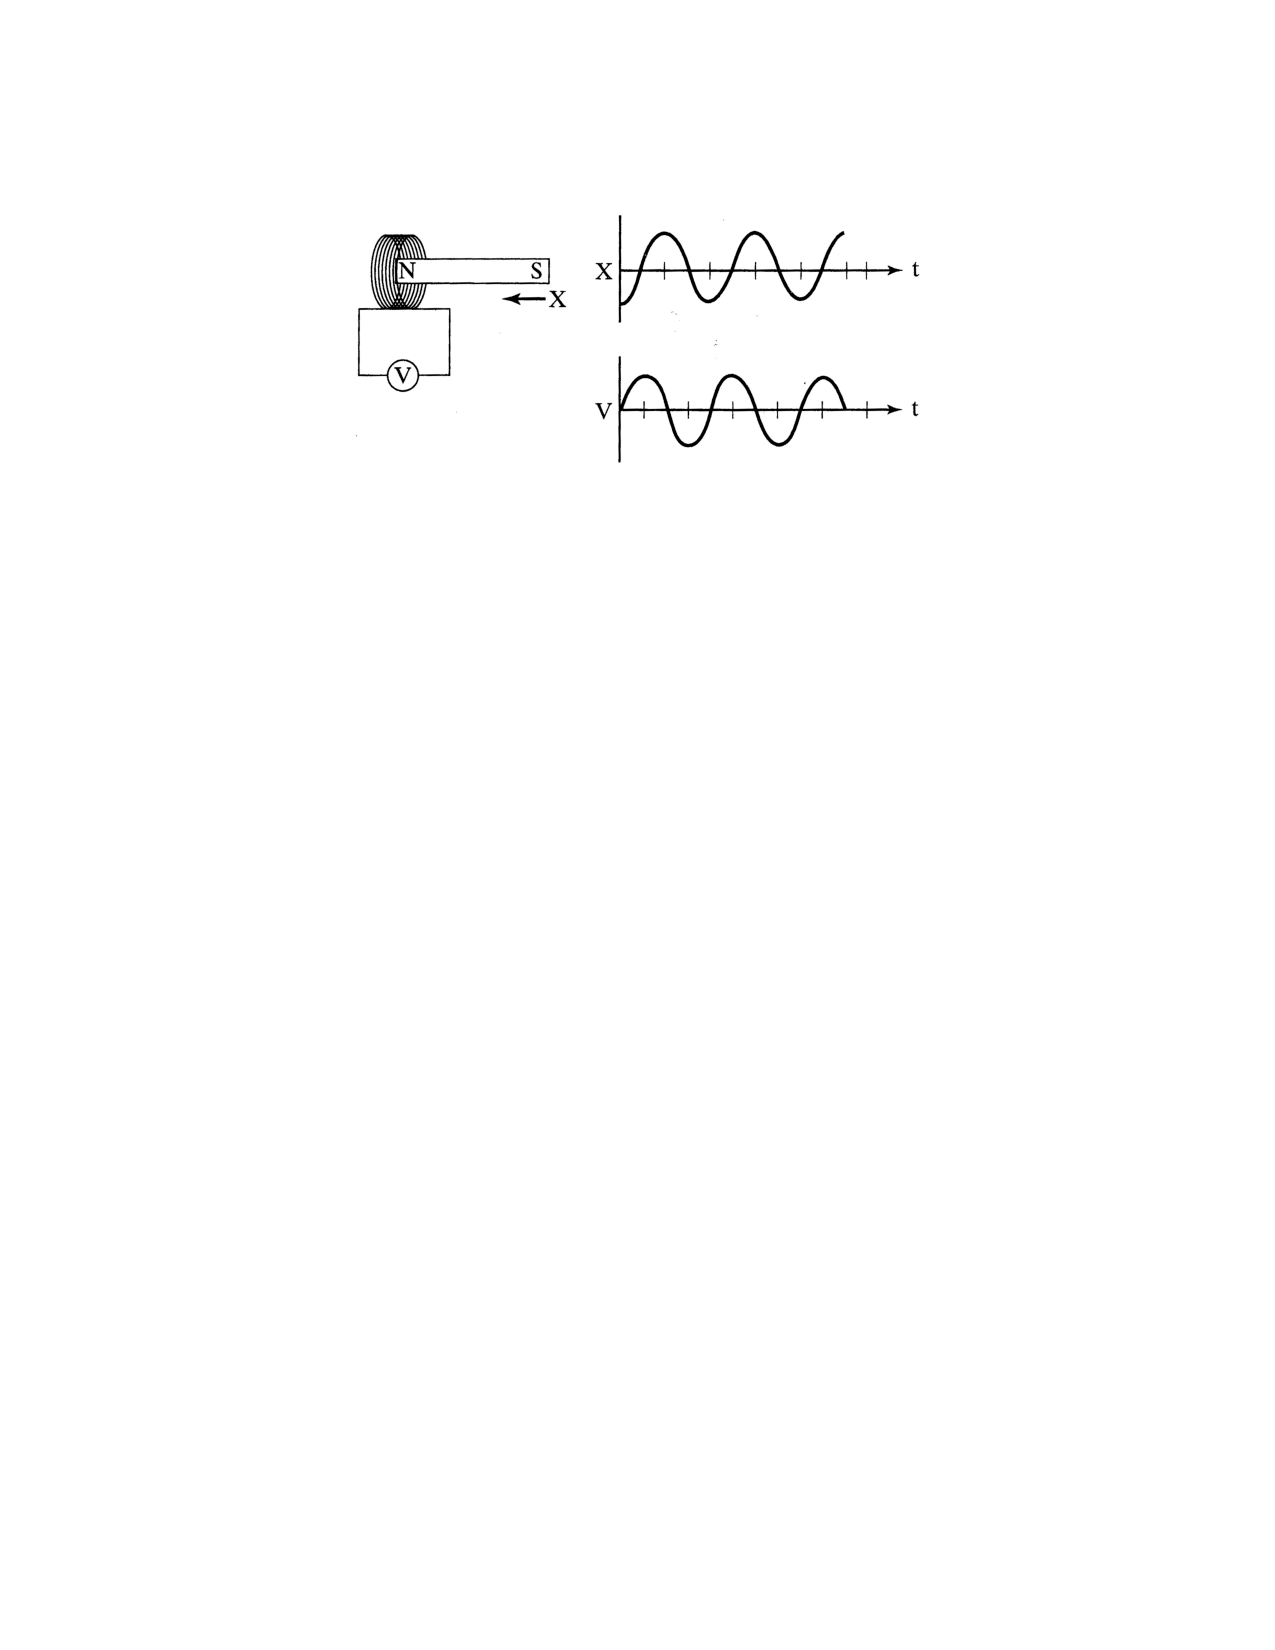
\includegraphics[width=0.6\textwidth]{faraday}
\caption{Illustration of Faraday's law.
As a magnetic moves back and forth ($X$ vs $t$) in the vicinty 
of a coil of wire, an alternating voltage ($V$ vs $t$) is induced
in the coil.
(Figure from ``Physics of Sound," by Berg and Stork.)} 
\label{f:faraday}
\end{center}
\end{figure}
%
 
\i Faraday's law of induction has had a profound influence of 
technology, as it underlies the operation of electric motors and generators.
It also underlies the operation of certain types of microphones and
loudspeakers (these will be described in the next subsection).

\i \underline{Demonstrations}:

(i) Illustrate how a hand-powered AC generator works.

(ii) Illustrate the operation of a simple DC motor constructed
from electromagnets.

(iii) Show a ``do-it-yourself" DC motor constructed from a D-cell
flashlight battery, a small magnet, paper clips, and a coil of (magnet)
wire stripped on one side.

\i Note that electric motors and electric generators are basically 
``inverses" of one another:

\underline{Electric generator}: 
mechanical energy is converted to electrical energy
by physically rotating a coil in an external magnetic field. 
An voltage is induced in the coil by Faraday's law.

\underline{Electric motor}: 
electrical energy is converted to mechanical energy 
by sending a current through a coil of wire.  
This current creates an electromagnet, which interacts with the 
external magnetic field, causing the coil to rotate.

\ei

%%%%%%%%%%%%%%%%%%%%%%%%%%%%%%%%%%%%%%%%%%%%%%%%%%%%%%%%%%%
\subsection{Microphones and loudspeakers}

\bi

\i Faraday's law of electromagnetic induction also underlies the
operation of so-called ``dynamic" microphones and loudspeakers.

\i A schematic diagram of a dynamic microphone is shown in 
Figure~\ref{f:microphone}.
%
\begin{figure}[htbp]
\begin{center}
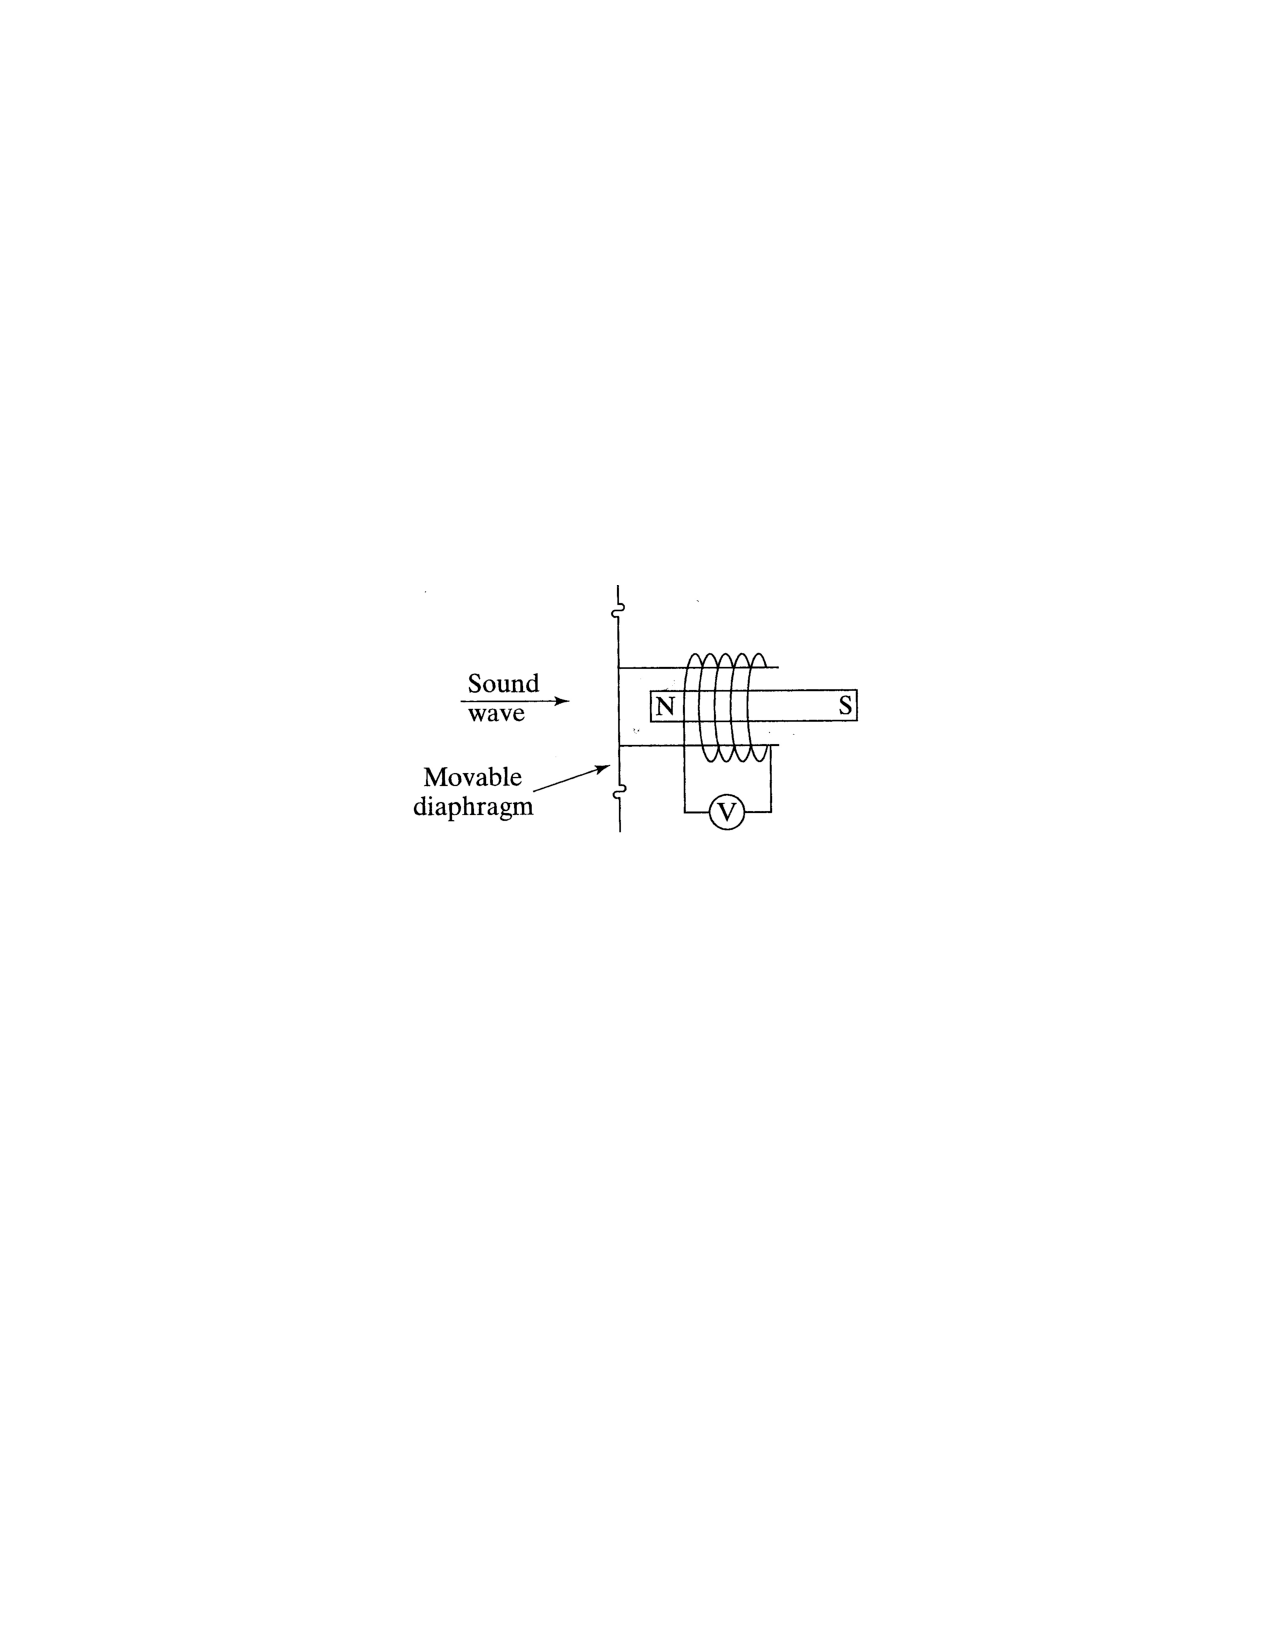
\includegraphics[width=0.5\textwidth]{microphone}
\caption{Schematic diagram of a dynamics microphone.
The pressure deviations associated with a sound wave
push back and forth on the diaphragm of the microphone.
A coil of wire, which is attached to the diaphragm, 
thus moves in the presence of a magnetic field.
The changing magnetic flux through the coil induces a voltage 
$V$ in the coil which follows the fluctuations of the sound wave.
(Figure from ``Physics of Sound," by Berg and Stork.)} 
\label{f:microphone}
\end{center}
\end{figure}
%

\i When a sound wave impinges on the movable diaphragm, 
the pressure deviations in the wave cause the diaphragm 
to move back-and-forth in response to the sound.
A coil of wire, which is attached to the diaphragm, thus 
moves with respect to a fixed magnetic field, inducing a
time-varying voltage in the coil (according to Faraday's
law) that follows the pressure deviations in the sound wave.
This voltage can then be amplified and used as input 
to other electronics that record or transmit the sound. 

\i A loudspeaker works like a microphone in reverse, see
Figure~\ref{f:loudspeaker}.
%
\begin{figure}[htbp]
\begin{center}
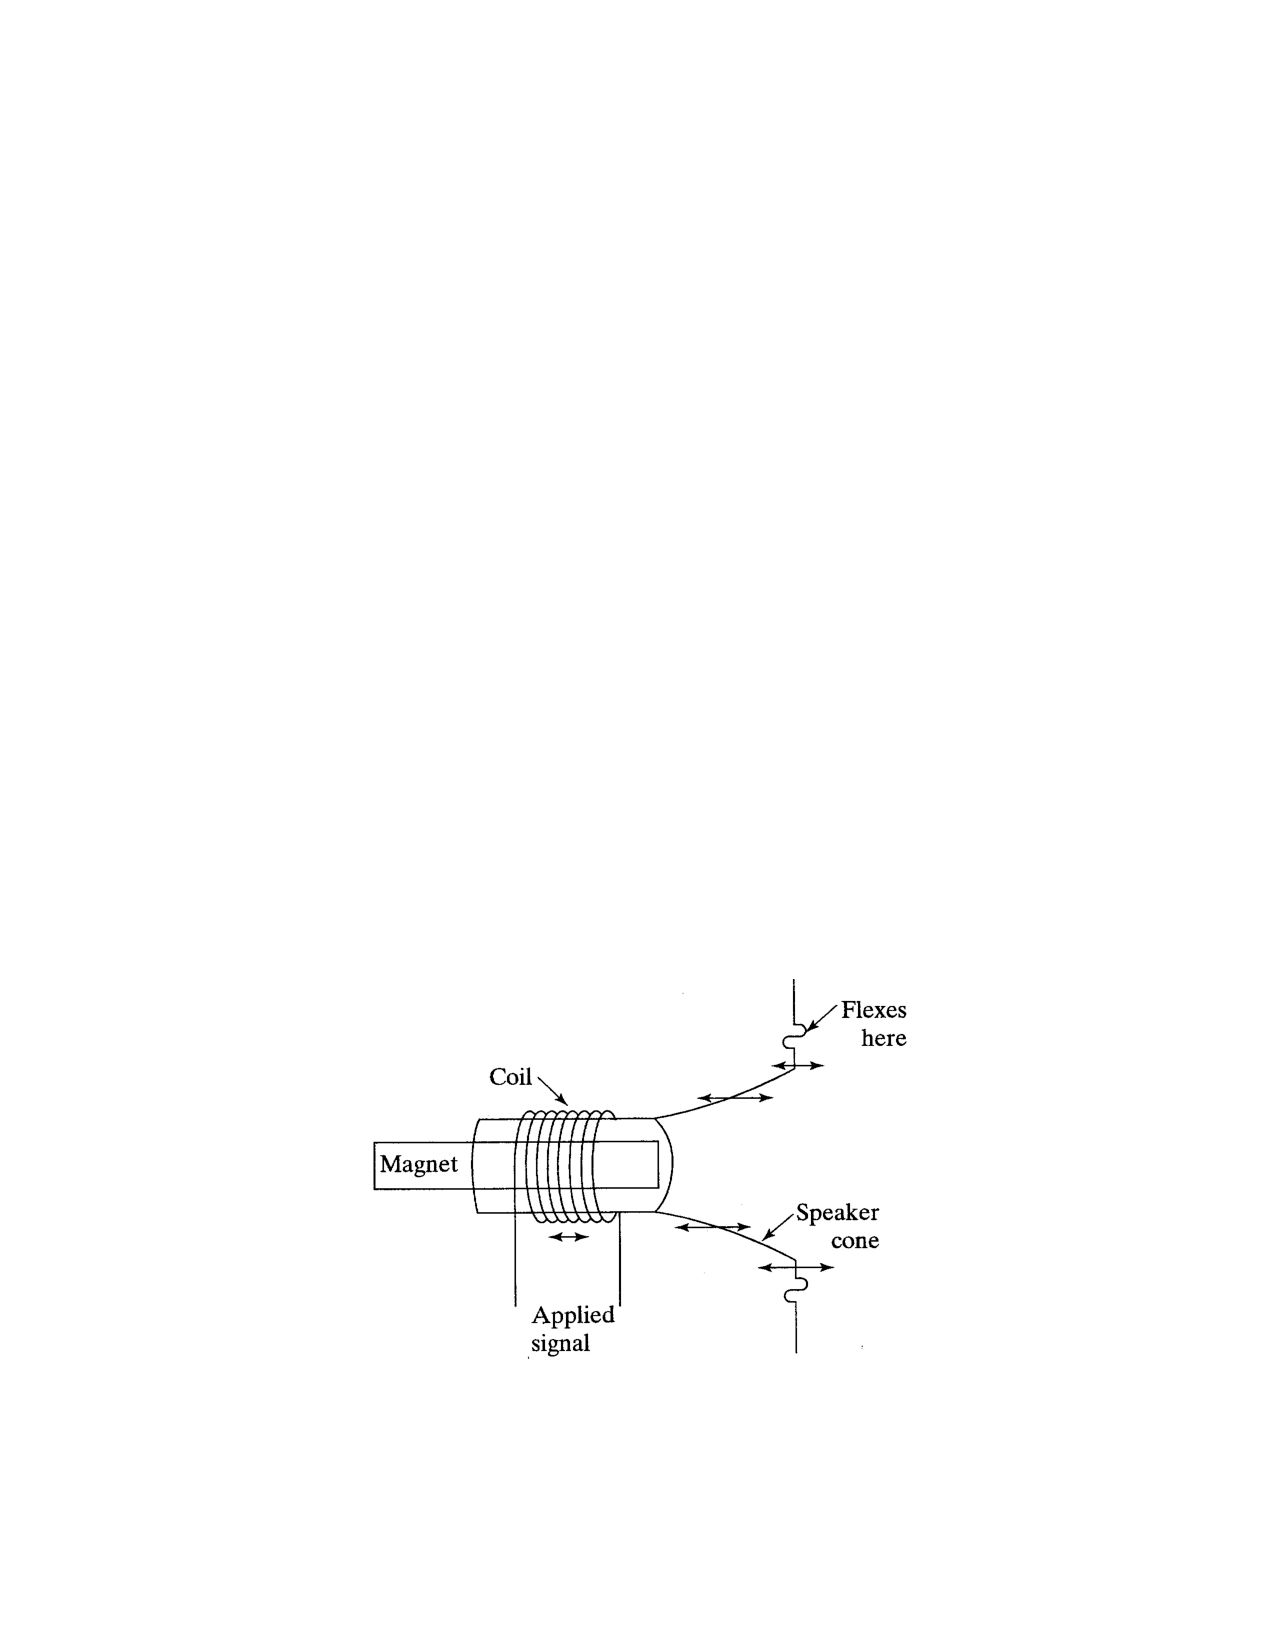
\includegraphics[width=0.5\textwidth]{loudspeaker}
\caption{An time-varying electrical signal (e.g., a voltage) 
applied to the coil creates a magnetic field that interacts 
with that of the permanent magnet.
The speaker cone, which is attached to the coil, 
moves back-and-forth in repsonse to this interaction,
thus producing a sound wave. 
(Figure from ``Physics of Sound," by Berg and Stork.)} 
\label{f:loudspeaker}
\end{center}
\end{figure}
%

\i A time-varying voltage, which is an electrical 
representation of the sound, is applied to a coil of wire 
that is attached to the loudspeaker cone.
A current then flows in this coil creating an electromagnet
that interacts with an external magnetic field, causing
the loudspeaker cone to move back-and-forth.
This motion creates pressure deviations in 
the air, which is the sound wave that we then hear.

\i The left and middle panels of Figure~\ref{f:loudspeaker_tunedport}
show two typical loudspeakers: 
(i) an ``acoustic suspension" loudspeaker, which is just 
a loudspeaker cone and coil suspended inside a closed box; and 
(ii) a ``tuned-port" loudspeaker, which is an acoustic
suspension loudspeaker whose box has a hole in it, which 
emphasizes the lower (bass) frequencies.
%
\begin{figure}[htbp]
\begin{center}
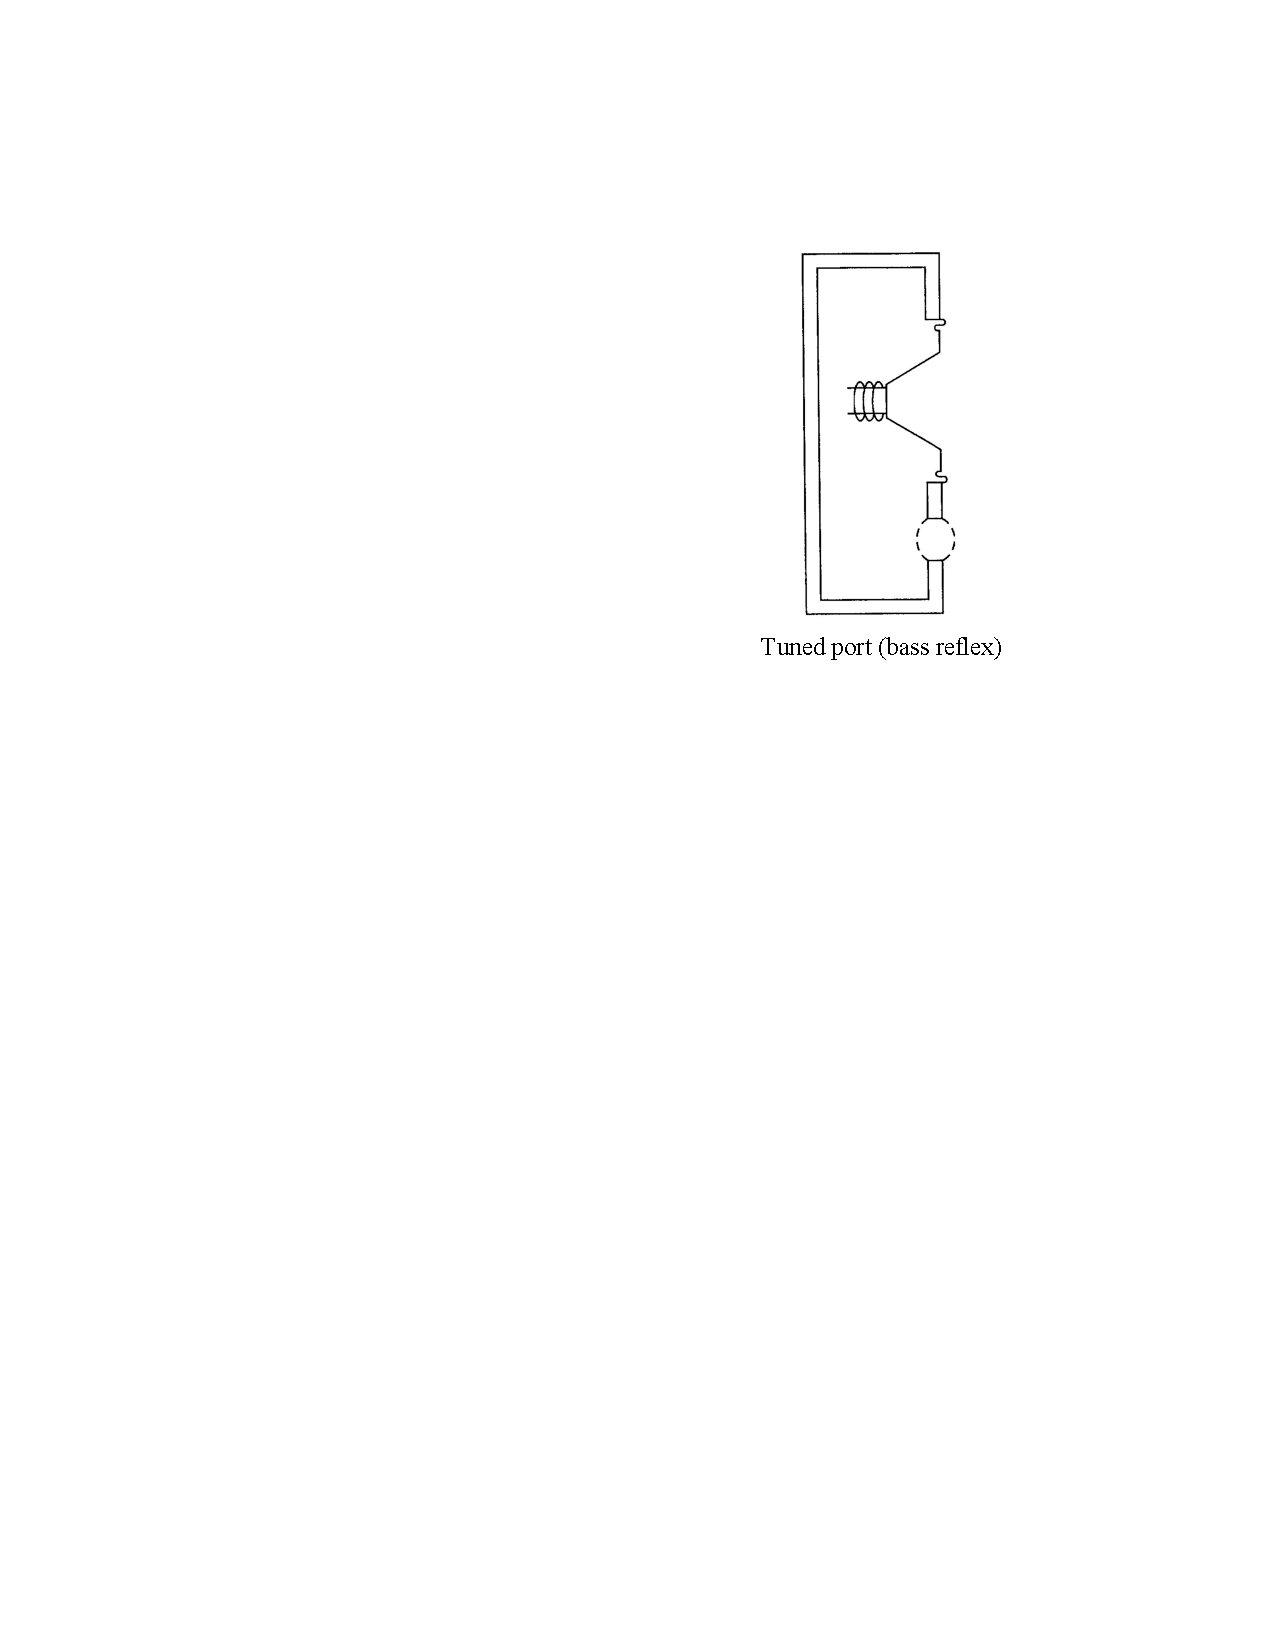
\includegraphics[height=0.4\textwidth]{loudspeaker_tunedport}
\hspace{0.2in}
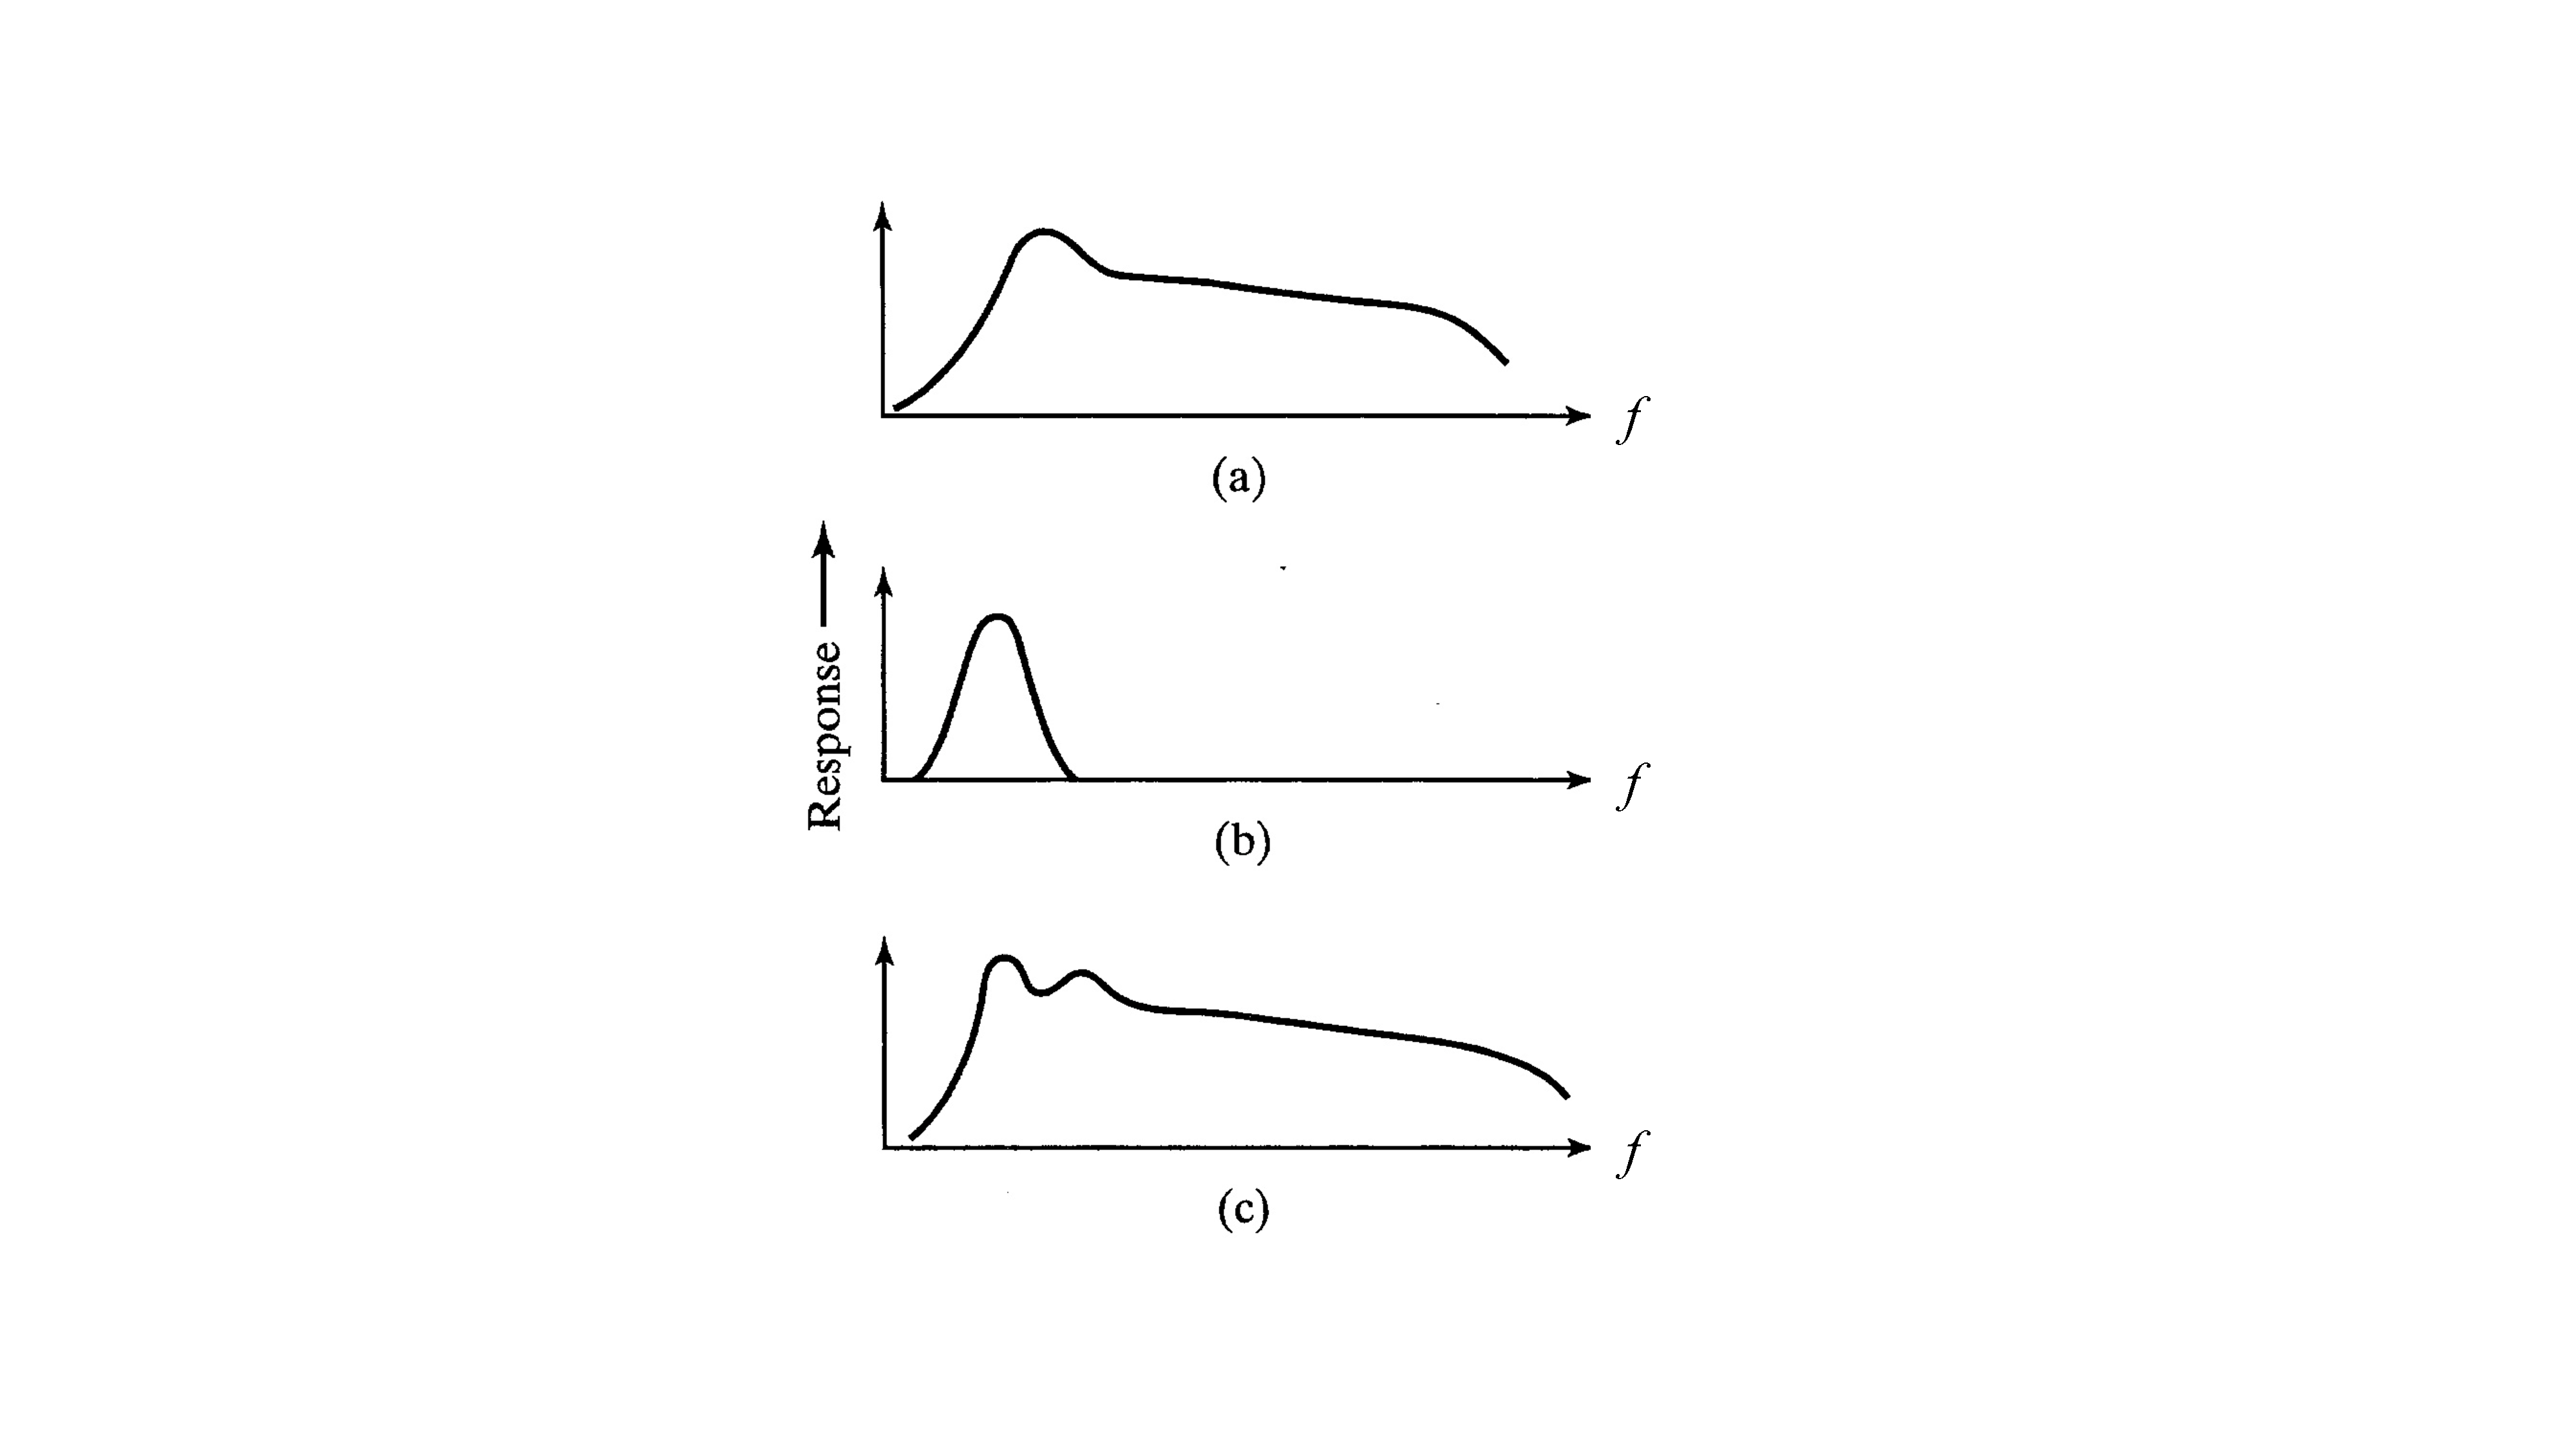
\includegraphics[height=0.4\textwidth]{loudspeaker_tunedport_response}
\caption{Acoustic-suspension and tuned-port loudspeakers (left, middle); 
frequency response curves (right).
(a) Frequency repsonse for an acoustic-suspension loudspeaker.
(b) Frequency response of an empty box with a hole (tuned port), 
which acts like a Helmholtz resonator.
(c) Combined frequency response for a tuned-port loudspeaker.
(Figures from ``Physics of Sound," by Berg and Stork.)} 
\label{f:loudspeaker_tunedport}
\end{center}
\end{figure}
%

\i The right-hand side of Figure~\ref{f:loudspeaker_tunedport}
shows the frequency response curves for the two loudspeakers:
(a) the frequency response of the acoustic-suspension loudspeaker;
(b) the frequency response of an empty box with a hole in it,
which acts like a Helmholtz resonator; and 
(c) the frequency response of the tuned-port speaker, which is
a combination of the frequency response curves shown in (a) and (b).

\i Compared to the acoustic-suspension loudspeaker, the tuned-port
loudspeaker is better at producing lower (bass) frequency sounds.
Without the hole, the suspension box would need to be larger for 
the loudspeaker to produce these lower frequencies.

\ei
